\documentclass[a4paper,10pt]{book}

\usepackage{color}
\usepackage{bm}
\usepackage{amsmath}
\usepackage{appendix}
\usepackage{xspace}
\usepackage{a4wide}
\usepackage{wrapfig}
\usepackage[numbers,comma,sort&compress]{natbib}
\usepackage{graphicx}
%\usepackage{xstring}
\usepackage{listings,xcolor,courier}
%\usepackage{draftcopy}
\usepackage{longtable}
\usepackage{paralist}
%\usepackage{fancyvrb}
\usepackage{listings}

\usepackage
[dvips, %or dvips or pdftex
pagebackref, %or backref
colorlinks=true,
linkcolor=webgreen, %defined below
filecolor=webbrown, %defined below
citecolor=webgreen, %defined below
pdftitle={VOTCA-CT manual},
pdfauthor={},
pdfsubject={VOTCA-CT},
pdfkeywords={charge transport organic semiconductors},
bookmarksopen=false,
pdfpagemode=UseNone]{hyperref}

\definecolor{webgreen}{rgb}{0,.5,0}
\definecolor{webbrown}{rgb}{.6,0,0}
\pdfcompresslevel=9

\usepackage[T1]{fontenc}
%\usepackage{times}
\usepackage{type1cm}

\input{hgid}

\newcommand{\equ}[1]{eq.~\eqref{equ:#1}}
\newcommand{\Equ}[1]{Eq.~\eqref{equ:#1}}
\newcommand{\fig}[1]{figure~\ref{fig:#1}}
\newcommand{\Fig}[1]{Figure~\ref{fig:#1}}
\newcommand{\sect}[1]{section~\ref{sec:#1}}

\newcommand{\slink}[2]{\hyperref[#1]{#2}}


\newcommand{\xml}{XML\xspace}
\newcommand{\gromacs}{GROMACS\xspace}
\newcommand{\gaussian}{GAUSSIAN\xspace}
\newcommand{\turbomole}{TURBOMOLE\xspace}
\newcommand{\tinker}{TINKER\xspace}
\newcommand{\dipro}{DIPRO\xspace}

\newcommand{\Alq}{$\mathrm{Alq}_3$\xspace}
\newcommand{\dcvt}{DCV2T\xspace}

\newcommand{\xyz}{\texttt{geometry.xyz}\xspace}
\newcommand{\orb}{\texttt{zindo.orb}\xspace}
\newcommand{\votcactp}{{\MakeUppercase{votca-ctp}}\xspace}

\newcommand{\calculator}{\hyperref[sec:calculators]{calculator}\xspace}

\newcommand{\xmloptions}{\texttt{options.xml}\xspace}
\newcommand{\xmlcsg}{\hyperref[sec:xmlmap]{\texttt{map.xml}}\xspace}
\newcommand{\xmlsegments}{\hyperref[sec:xmlsegments]{\texttt{segments.xml}}\xspace}
\newcommand{\sqlstate}{\hyperref[sec:statefile]{\texttt{state.db}}\xspace}
\newcommand{\topology}{\texttt{topol.tpr}\xspace}
\newcommand{\trajectory}{\texttt{traj.xtc}\xspace}

\newcommand{\opt}{\texttt{{ -}o}\xspace}
\newcommand{\seg}{\texttt{{ -}s}\xspace}
\newcommand{\sql}{\texttt{{ -}f}\xspace}
\newcommand{\exe}{\texttt{{ -}e}\xspace}
\newcommand{\tpl}{\texttt{{ -}t}\xspace}
\newcommand{\csg}{\texttt{{ -}m}\xspace}
\newcommand{\trj}{\texttt{{ -}c}\xspace}


\newcommand{\refcalc}{\hyperref[ref:calculators]{calculators}\xspace}

\newcommand{\overlap}{\hyperref[prog:moo_overlap]{\texttt{moo\_overlap}}\xspace}
\newcommand{\ctprun}{\hyperref[prog:ctp_run]{\texttt{ctp\_run}}\xspace}
\newcommand{\ctpmap}{\hyperref[prog:ctp_map]{\texttt{ctp\_map}}\xspace}
\newcommand{\ctpdipro}{\hyperref[prog:ctp_dipro]{\texttt{ctp\_dipro}}\xspace}

\newcommand{\sqlite}{\texttt{sqlite3}\xspace}
\newcommand{\sqlconjsegproperties}{\texttt{conjseg\_properties}\xspace}
\newcommand{\sqlconjsegs}{\texttt{conjsegs}\xspace}
\newcommand{\sqlmolecules}{\texttt{molecules}\xspace}
\newcommand{\sqlpairintegrals}{\texttt{pairintegrals}\xspace}
\newcommand{\sqlpairproperties}{\texttt{pairproperties}\xspace}
\newcommand{\sqlpairs}{\texttt{pairs}\xspace}
\newcommand{\sqlrigidfragproperties}{\texttt{rigidfrag\_properties}\xspace}
\newcommand{\sqlrigidfrags}{\texttt{rigidfrags}\xspace}
\newcommand{\sqlframes}{\texttt{frames}\xspace}


\newcommand{\suggestion}[1]{{\color{red}SUGGESTION: #1}}

\newcommand{\segmentref}[1]{segments.#1}
\newcommand{\segmentopt}[1]{\hyperlink{\segmentref{#1}}{\StrSubstitute{#1}{_}{\_}}\xspace}
\newcommand{\calcref}[1]{#1}
\newcommand{\calcopt}[1]{\hyperlink{\calcref{#1}}{\StrSubstitute{#1}{_}{\_}}\xspace}

\newcommand{\calc}[1]{\hyperref[calc:#1]{\texttt{#1}}\xspace}

\def\bibsection{%
    \chapter*{Bibliography}%
    \addcontentsline{toc}{chapter}{Bibliography}
}

\renewcommand*{\showkeyslabelformat}[1]{{\normalfont\tiny\sffamily#1}}
\definecolor{refkey}{rgb}{1,0,0}
\definecolor{labelkey}{rgb}{1,0,0}


\begin{document}
\frontmatter
\begin{titlepage}

\center{\fontsize{4cm}{5cm}\selectfont VOTCA}
\center{\fontsize{1.5cm}{3cm}\selectfont USER MANUAL}

\vspace*{3cm}
\center{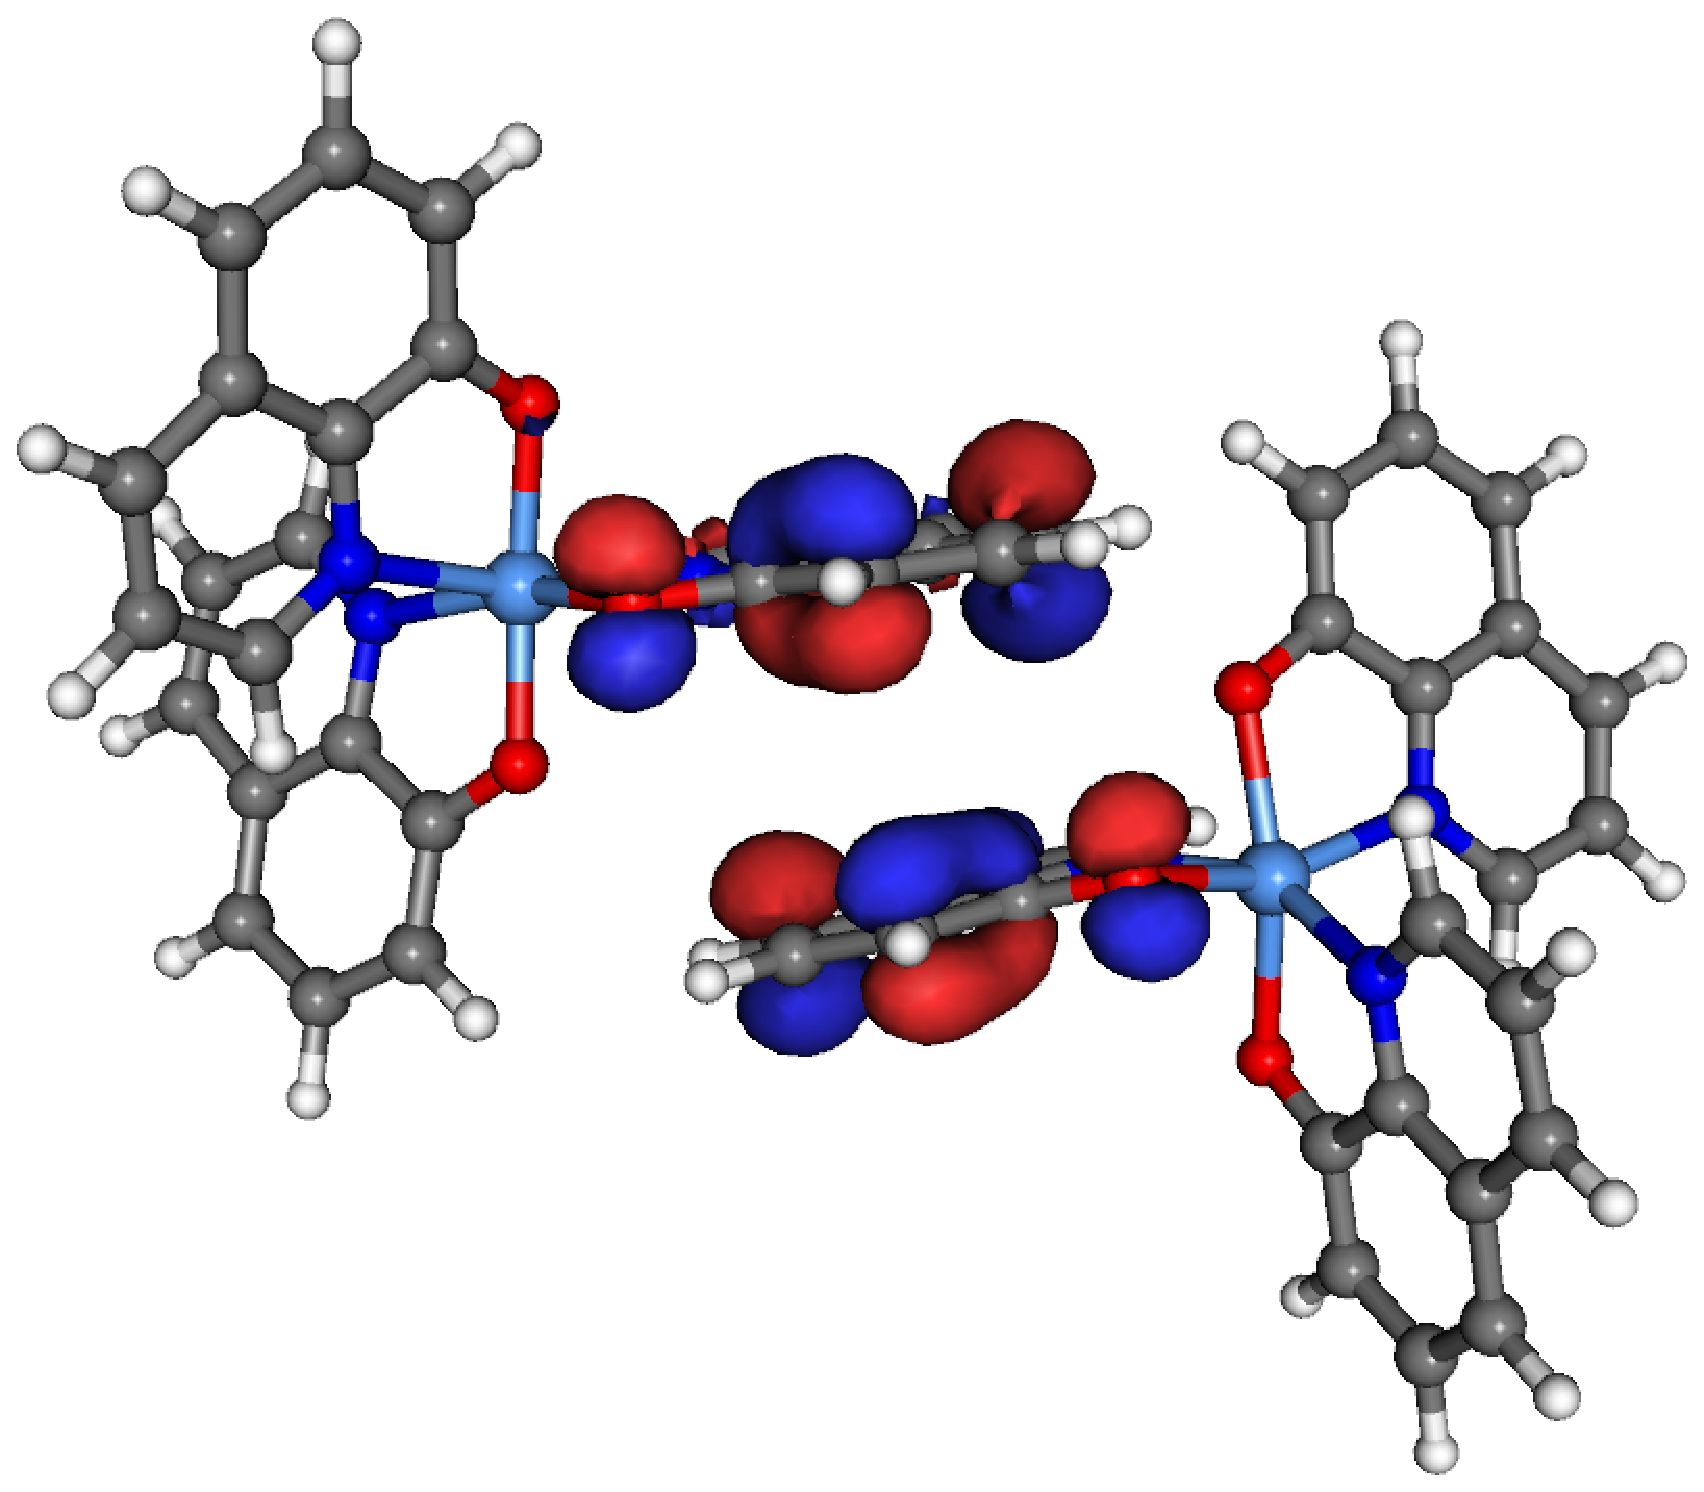
\includegraphics[width=\columnwidth]{fig/logo}}
\vspace*{1cm}
\vfill
\vspace*{1.4cm}
\center{\large{\today}}
\vspace*{-0.3cm}
\center{\footnotesize{Version: \gitid}}
\center{\footnotesize{Programs version: \csgid}}

\vspace*{1cm}
%\center{
\large{\copyright \hspace*{0.1cm} VOTCA development team}
%}
\vspace*{0.5cm}

\htmladdnormallink{\color{black}\large{www.votca.org}}{http://www.votca.org}
\end{titlepage}

\section*{Disclamer}
This manual is not complete. The best way to start using the software is to look at provided tutorials. The reference section is generated automatically from the source code, so please make sure that your software and manual versions match.  

\section*{Citations}
Development of this software depends on academic research grants. If you are using the package, please cite the  following papers \\

\vspace{0.1cm}
\noindent
\cite{mashayakrelative} Relative entropy and optimization-driven coarse-graining methods in VOTCA, \\
S.Y. Mashayak, Mara Jochum, Konstantin Koschke, N.R. Aluru, Victor R\"uhle, and Christoph Junghans,\\
\htmladdnormallink{  {\itshape Plos One} (2015)}
{http://dx.doi.org/10.1371/journal.pone.0131754}

\vspace{0.1cm}
\noindent
\cite{ruhle2011hybrid} Hybrid approaches to coarse-graining using the VOTCA package: liquid hexane, \\
Victor R\"uhle and Christoph Junghans, \\
\htmladdnormallink{  {\itshape Macromol. Theory Simul.} 20, 472 (2011)}
{http://dx.doi.org/10.1002/mats.201100011}

\vspace{0.1cm}
\noindent
\cite{Ruehle:2009.a} Versatile Object-oriented Toolkit for Coarse-graining Applications \\
Victor R\"uhle, Christoph Junghans, Alexander Lukyanov, Kurt Kremer, and Denis Andrienko \\
\htmladdnormallink{  {\itshape J. Chem. Theor. Comp.} 5, 3211, 2009}
{http://dx.doi.org/10.1021/ct900369w}

\section*{Development}
The core development is currently taking place at the Los Alamos National Laboratory and Max Planck Institute for Polymer Research, Mainz, Germany.

\section*{Copyright}
\votca is free software. The entire package is available under the Apache License. For details, check
the LICENSE file in the source code. The \votca source code is available on our homepage, \htmladdnormallink{\color{black}www.votca.org}{http://www.votca.org}.

\vfill

\thispagestyle{empty}
\cleardoublepage

\tableofcontents
\cleardoublepage
\mainmatter
\chapter{Introduction}
\label{sec:introduction}

Charge carrier dynamics in an organic semiconductor can often be described in terms of charge hopping between localized states. The hopping rates depend on electronic coupling elements, reorganization energies, and driving forces, which vary as a function of position and orientation of the molecules.  The exact evaluation of these contributions in a molecular assembly is computationally prohibitive. Various, often semi-empirical, approximations are employed instead. The purpose of \votcactp is to simplify the workflow for charge transport simulations, provide a uniform error-control for the methods, flexible platform for their development, and eventually allow in silico pre-screening of organic semiconductors for specific applications. 

The toolkit is implemented using modular concepts introduced earlier in the Versatile Object-oriented Toolkit for Coarse-graining Applications (VOTCA)~\cite{ruehle_versatile_2009}. The VOTCA structures are adapted to reading atomistic trajectories, mapping them onto conjugated segments and rigid fragments, and substituting (if needed) rigid fragments with the optimized copies. 

The \hyperref[sec:moo]{molecular orbital overlap} module calculates electronic coupling elements between  conjugated segments from the corresponding molecular orbitals. It relies on the semi-empirical INDO Hamiltonian and molecular orbitals in the format provided by the \gaussian package. An alternative,  \hyperref[sec:dft]{density-functional based approach}, has interfaces to the \gaussian and \turbomole packages. An interface to the \tinker package is provided for calculations of electrostatic and polarization contributions to energetic disorder. 

The  \hyperref[sec:kmc]{kinetic Monte Carlo module} reads in the neighbor list, site coordinates, and hopping rates and performs charge dynamics simulations using either periodic boundary conditions or charge sources and sinks. 

The toolkit is written as a combination of modular C++ code and scripts. The data transfer between programs is implemented via a state file or database, which is also used to restart simulations. Analysis functions and most of the calculation routines are encapsulated by using the observer pattern~\cite{gamma_design_1995} which allows the implementation of new functions as individual modules.
\chapter{System morphology}
\label{sec:morphology}

In this section we describe how to specify the morphology of the system. We will use DCV2T as an example.

\section{Single molecule}

\begin{wrapfigure}{ht}{0.5\linewidth}
\centering
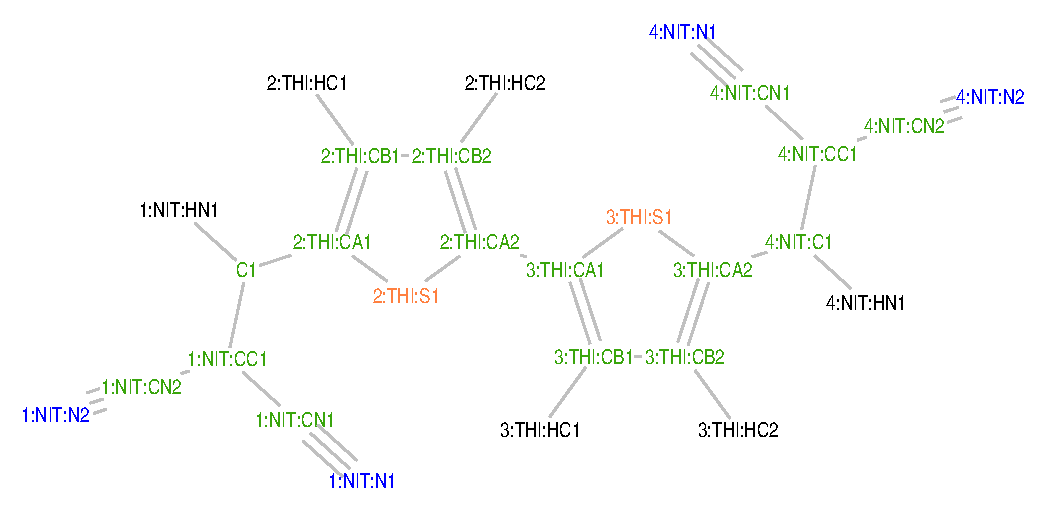
\includegraphics[width=0.9\linewidth]{./fig/chemical_structure/dcv2t_atom_types}
\caption{\small Atom types of DCV2T. The molecule consists of two building blocks (residues): thiophene (THI) and dicyanovinyl (NIT). }
\label{fig:dcv2t_at}
\end{wrapfigure}

%\clearpage
The structure of DCV2T, together with atom type definitions, is shown in fig.~\ref{fig:dcv2t_at}. DCV2T is a typical donor-acceptor-type molecule, with two electron-donating thiophene and two electron-withdrawing dicyanovinyl groups. The pdb file which contains residue types, residue numbering, atom names, atom types, and atom coordinates is shown below. In its ground state the molecule is practically planar. 

\section{Simulation box}
An amorphous morphology was obtained by quenching the 512 DCV2T molecules after equilibrating the system above the glass transition temperature. What we will need is a snapshot out of the trajectory and the topology file describing the system (all in GROMACS format).

\clearpage
\lstinputlisting[
  basicstyle=\ttfamily\footnotesize,
  frame=lines,
  identifierstyle=\color{red},
  keywordstyle=\color{blue},
  showstringspaces=false,
 label=list:pdb, 
 morekeywords={HETATM,THI,NIT},
 caption={pdb file of DCV2T}]%
{./fig/chemical_structure/dcv2t.pdb}

%\VerbatimInput[%
%frame=lines,
%framesep=4mm,
%label=\fbox{pdb file of DCV2T}, 
%framerule=0.5mm,
%rulecolor=\color{red},
%baselinestretch=1,
%fontsize=\footnotesize%,
%numbers=left
%]%
%{./fig/chemical_structure/dcv2t.pdb}

\section{Mapping definitions}
{\em Mapping definitions} describe how to map a single molecule from atomistic to coarse-grained representation. The mapping definition have only to be specified once per molecule. The file contains sections for coarse-grained beads, bonded interactions in coarse grained scheme as well as mapping matrices. 

\subsection{Example - mapping file for propane}

\lstinputlisting[frame=single,caption=Mapping for propane]{functionality/propane.xml}

\chapter{Transfer Integrals}

\section{Semi-empirical}

\section{Density-functional}

\includegraphics[width=0.4\linewidth]{fig/complicated}

\chapter{Manual pages}
%
% if you want to refer to any of the tags specified here use the following command
% \segmentopt{crgunit_type.ChargeUnitType.posname}
%
\section{Programs}
\label{ref:programs}
\input{reference/programs/all}

\section{Calculators}
\label{ref:calculators}
\label{sec:calculators}

Calculator is a piece of code which computes specific system properties, such as site energies, transfer integrals, etc. \ctprun is a wrapper program which executes all calculators. The generic syntax is 

  \ctprun \exe \texttt{"calc1, calc2, ..."} \opt \xmloptions
\vskip 0.2cm
%
File \xmloptions lists all options needed to run a specific calculator. The format of this file is explained in listing~\ref{list:calc}. A complete list of calculators is given in the \refcalc reference section.
%
\lstinputlisting[label=list:calc, 
 caption={\small A part of the \xmloptions file with options for the \texttt{calculator\_name\{1,2\}} \refcalc.
}]{./reference/calculators.xml}

\input{reference/calculators/all}
\vfill

\section{Options}
\label{ref:options}
%\setdefaultleftmargin{0.8em}{0.8em}{0.8em}{0.8em}{0.8em}{0.8em}

\subsection{Mapping file}
\rowcolors{1}{invisiblegray}{white}
{\small 
\input{reference/xml/map.xml}
}
\vfill

\subsection{Conjugated segments}
\rowcolors{1}{invisiblegray}{white}
{\small 
\input{reference/xml/segments.xml}
}
\vfill

\subsection{Calculator options}
\rowcolors{1}{invisiblegray}{white}
{\small 
\input{reference/xml/options.xml}
}
\vfill


\bibliographystyle{unsrt}
%\bibliography{votca}

\end{document} 
